\section{The BFW Benchmark and Dataset}


We now discuss the \gls{bfw} dataset (\ie collection and preparation), along with the evaluation protocols. We conclude this section by reviewing the settings followed to survey bias in humans.

\subsection{The data}
Problems of bias in \gls{fr} motivated us to build \gls{bfw}. The data evenly represent various subgroups partitioned by demographic. Inspired by \gls{dp}~\cite{demogPairs}, the specification of \gls{bfw} follows in suit, but with additional subgroups (\ie \gls{if} and \gls{im}), an increase in the number of subjects per subgroup, and many more pairs (Table~\ref{tab:ethnic-splits}). 




\vspace{1mm}
\noindent\textbf{Compiling subject list.} 
Subjects were sampled from VGG2~\cite{Cao18} - unlike others built from multiple sources, \gls{bfw} has fewer potential conflicts in train and test overlap with existing models. We used pre-trained ethnicity~\cite{ambekar2009name} and gender~\cite{levi2015age} classifiers to find candidates for the different subgroups.



\vspace{1mm}
\noindent\textbf{Detecting faces.} Faces were detected using MTCNN~\cite{zhang2016joint}.\footnote{\href{https://github.com/polarisZhao/mtcnn-pytorch}{https://github.com/polarisZhao/mtcnn-pytorch}} Then, assigned into one of two sets. Faces within detected bounding box (BB) regions extended out 130\% in each direction, with zero-padding as the boundary condition made-up one set. The second set were faces aligned and cropped for Sphereface~\cite{liu2017sphereface} (see the next step). Also, coordinates of the BB and the five landmarks from \gls{mtcnn} were stored as part of the static, raw data. For samples with multiple face detections, we used the BB area times the confidence score of the \gls{mtcnn} to determine the face most likely to be the subject of interest, with the others set aside and labeled \textit{miss-detection}. 



\vspace{1mm}
\noindent\textbf{Validating labels.} 
Faces of \gls{bfw} were encoded using the original implementation of the \gls{soa} Sphereface~\cite{liu2017sphereface}: applying an affine transformation to align faces according to predefined eye locations, each face fed through twice (\ie the original and horizontally flipped), with the final encoding obtained by fusing the two features by average pooling (\ie 512 D). A matrix of cosine similarity scores was then generated for each subject and removed samples (\ie rows) with median scores below threshold $\theta=0.2$ (set manually). Mathematically, the $n^{th}$ sample for the $j^{th}$ subject with $N_j$ faces was removed if the ordinal rank of its score $n = \frac{P\times N}{100}\geq\theta$, where $P=50$. In other words, the median (\ie 50 percentile) of all scores for a faces with respect to all of faces for the respective subject must pass a threshold of $\theta=0.2$; else, the face is dropped. This allowed us to quickly prune \gls{fp} face detections. Following~\cite{robinson2016families, robinson2018visual}, we built a JAVA tool to visually validate the remaining faces. For this, the faces were ordered by decreasing confidence, with confidence set as the average score, and then displayed as image icons on top toggling buttons arranged as a grid in a sliding pane window. Labeling then consisted of going subject-by-subject and flagging faces of \emph{imposters}.

\begin{figure}[!t] 
	\centering    
 \glsunset{fpr}
  \glsunset{fnr}
	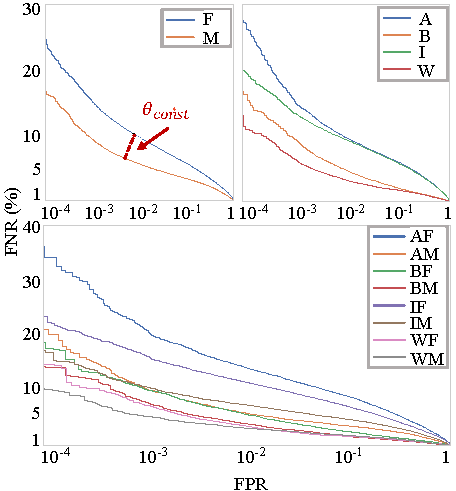
\includegraphics[width=.9\linewidth]{figures/detcurve-improved.pdf}
		\caption{\small{\textbf{\gls{det} curves.} \emph{Top-left}: per gender. \emph{Top-right}: per ethnicity. \emph{Bottom}: per subgroup (\ie combined). Dashed line shows about 2$\times$ difference in \gls{fpr} for the same threshold $\theta_{const}$. \gls{fnr} is the match error count (closer to the bottom is better).}}
		\glsreset{det}\glsreset{fpr}
\label{fig:detcurves} 
\end{figure} 
%\vspace{1mm}
\noindent\textbf{Sampling faces and creating folds.} We created lists of pairs in five-folds with subjects split evenly per subject and without overlap across folds. Furthermore, a balance in the number of faces per was obtained by sampling twenty-five faces at random from each. Next, we generated a list of all the face pairs per subject, resulting in $\sum_{l=1}^{L}\sum_{k=1}^{K_d} {N_k \choose 2}$ positive pairs, where the number of faces of all $K_l$ subjects $N_k=25$  for each of the $L$ subgroups (Table~\ref{tab:ethnic-splits}). Next, we assigned subjects to a fold. To preserve balance across folds, we sorted subjects by the number of pairs and then started assigning to alternating folds from the one with the most samples. Note, this left no overlap in identity between folds. Later, a negative set from samples within the same subgroup randomly matched until the count met that of the positive. Finally, we doubled the number with negative pairs from across subgroups but in the same fold.

\begin{figure}[t!] 
	\glsunset{fpr}
% 	\glsunset{sdm}
	\centering
	\centering
	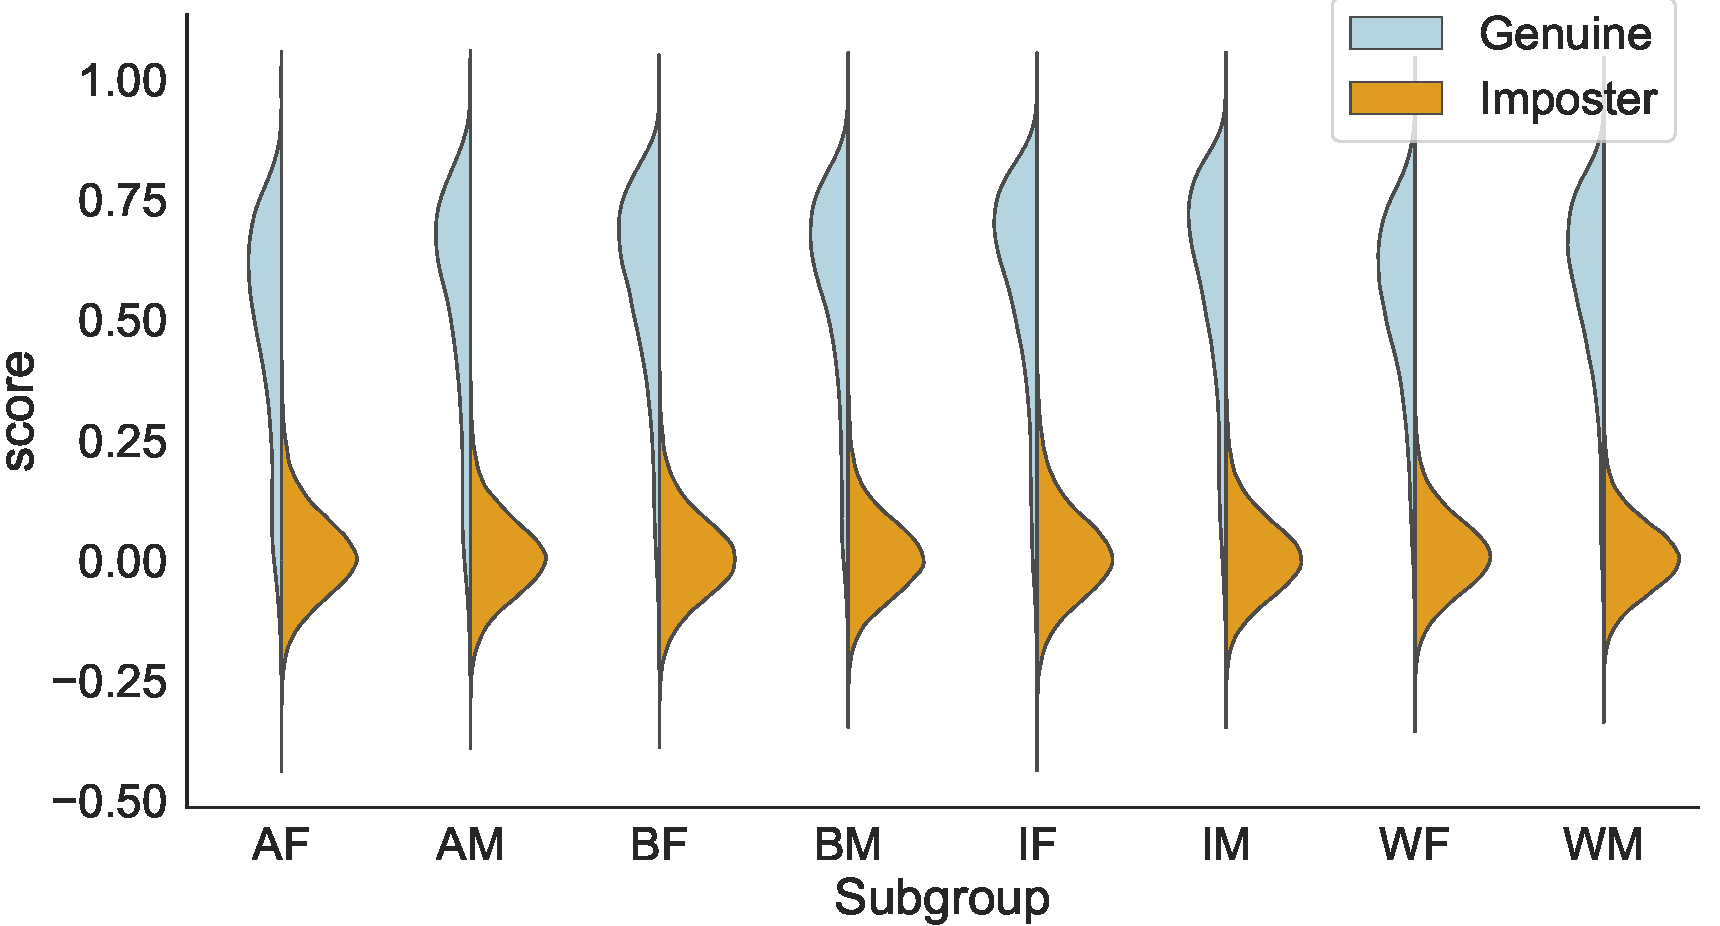
\includegraphics[width=1\linewidth]{figures/violinplots.pdf}
		\caption{\small{\textbf{\Gls{sdm} across subgroups.} Scores of \emph{imposters} have medians around 0.3 but with variations in upper percentiles; \emph{genuine} pairs vary in mean and spread (\eg \gls{af} has more area of overlap). A threshold varying across different subgroups yields a constant \gls{fpr}.}} \label{fig:detection-model} 
% 		\glsreset{sdm}
\end{figure} 

% \vspace{-5pt}
\subsection{Problem formulation}\label{subsec:pf} 
% \gls{lfw}~\cite{LFWTech}, a commonly used benchmark for ~\gls{fr}, reserves specific train-test face-pair lists. 
\Gls{fv} is the special case of the two-class (\ie boolean) classification. Hence, pairs are labeled as the ``same'' or ``different'' \textit{genuine} pairs (\ie \textit{match}) or \textit{imposter} (\ie \textit{mismatch}), respectively. This formulation (\ie \gls{fv}) is highly practical for applications like access control, re-identification, and surveillance. Typically, training a separate model for each unique subject is infeasible. Firstly, the computational costs compound as the number of subjects increase.  Secondly, such a scheme would require model retraining each time a new person is added. Instead, we train models to encode facial images in a feature space that captures the uniqueness of a face, to then determine the outcome based on the output of a scoring (or distance) function. Formally put:
\begin{equation}\label{eg:matcher}
    f_{boolean}(\vec{x}_i, \vec{x}_j) = d(\vec{x}_i, \vec{x}_j) \leq \theta,
\end{equation}

where $f_{boolean}$ is the \textit{matcher} of the feature vector $\vec{x}$ for the $i^{th}$ and $j^{th}$ sample~\cite{LFWTech}.

Cosine similarity is used as the \emph{matcher} in Eq~\ref{eg:matcher} the closeness of $i^{th}$ and $j^{th}$ features, \ie
$
s_l= \frac{f_i\cdot f_j}{||f_i||_2||f_j||_2}
$ is the closeness of the $l^{th}$ pair. 

\begin{figure}[t!]
	\centering    
	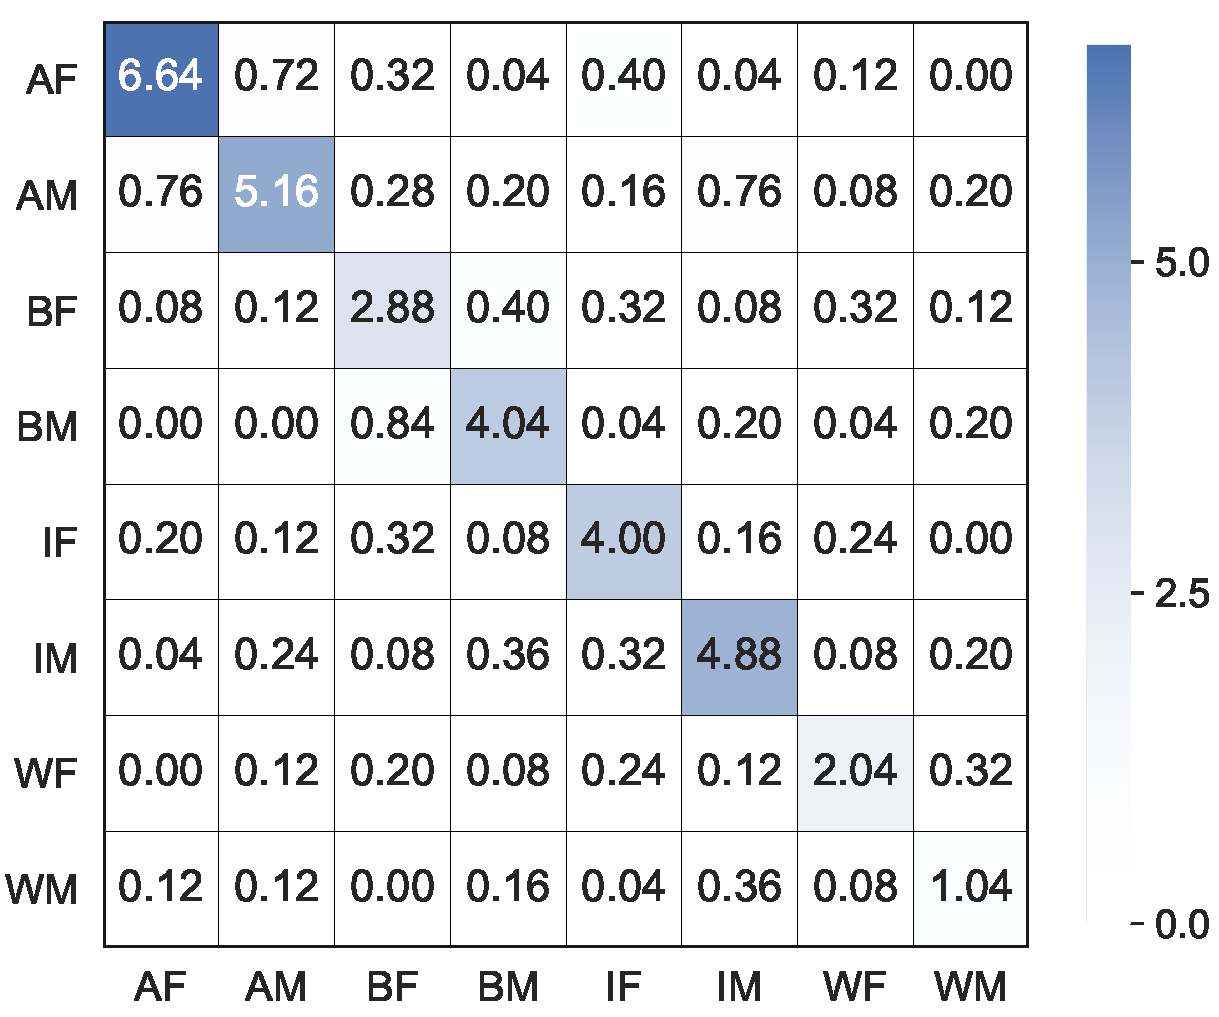
\includegraphics[width=.75\linewidth]{figures/confusion.pdf}
		\caption{\small{\textbf{Confusion matrix.} Error (Rank 1, \%) for all faces of \gls{bfw} vs. all others. Error concentrates intra-subgroup - consistent with the \gls{sdm} (Fig.~\ref{fig:detection-model}), as \gls{af} performs the worst, mostly confused by \gls{af}. Although race/ethnicity are challenging to define, this shows the subgroups are meaningful for \gls{fr}.}}
		\label{fig:confusion} 
%		    \vspace{-6mm}
\end{figure} 

\subsection{Human assessment}\label{subsec:human-assessment}
To focus on the human evaluation experiment, we honed-in on pairs from two groups, white Americans (W) and Chinese from China (C). This minimized variability by only analyzing the subsets of the broader groups of whites and Asians. %We evaluated human on face pairs focusing on two subgroups: Chinese and Caucasians. 

Samples were collected by recruiting subjects from multiple sources (\eg social media, email lists, and family/friends)-- a total of 120 participants were sampled at random from all the submissions that were (1) complete and (2) from a W or C participant. Specifically, there were 60 W and 60 C, both with \gls{m} and \gls{f} split evenly. A total of 50 face pairs of non-famous ``look-alikes'' were collected from the internet, with 20 ({\emph WA}) and 20 ({\emph C}) pairs (male and female split evenly). The other 10 pairs are of others (\eg Hispanic/ Latino, Japanese, African). The survey was created, distributed, and recorded via \href{https://paperform.co}{PaperForm}. 
